	Conducting an interview involves moving backward and forward through a questionnaire since the logical states (filter, loop and check) can be visited multiple times. Every time those states are visited, it has to be guaranteed that the expression holds the appropiate result, i.e. reflects the latest changes from any of the operands that each variable referenced has. A naive approach, may perform an evaluation of the expression every time a state is reached but this behaviour may be improved if the observer pattern is considered.

	The observer pattern is addressed to notify observers when any property has changed. The figure \ref{fig:design:observerPattern} represents the behavioural pattern that we have applied for eliminating unnecessary operations. On one hand, the \emph{observable} (e.g. an operand object), contains several methods such as \emph{isUnary()} and \emph{isBinary()} to determine whether or not an operator passed is compatible with the operand. Or \emph{resolve()} methods that evaluate an intermediate operation either unary or binary against that observable. For instance, an operand integer holding 5 as value, will return 6 when the resolve method is called with the operator INC (unary). The same result will be obtained when the resolve method gets the arguments 1 and ADD (binary operator). The most important feature for this class is the value property which is updated through the setValue.

	\begin{figure}[H]
	\centering
	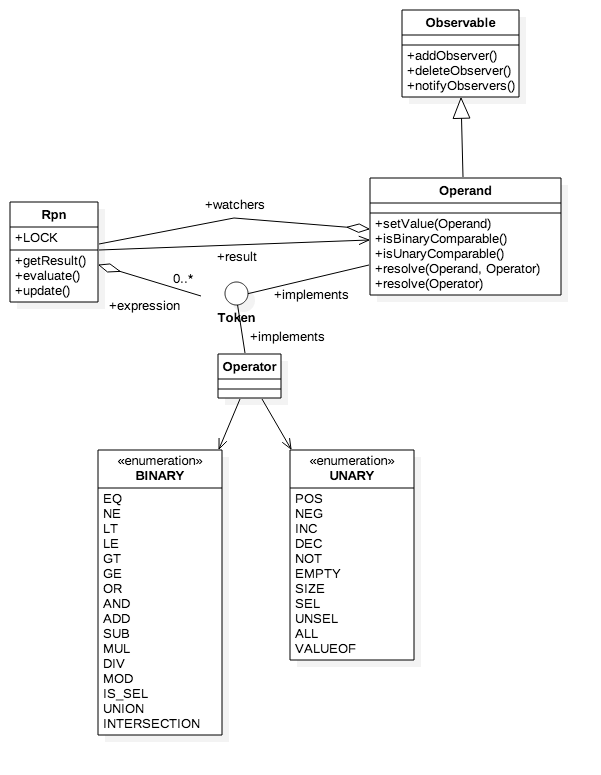
\includegraphics[max size={\textwidth}{\textheight}]{design/img/observer.png}
	\caption{Observer Design pattern for RPN expressions}
	\label{fig:design:observerPattern}
	\end{figure}

	On the other hand, the \emph{observer} (e.g. an \gls{rpn} object), which is defined for every pseudo state, contains two important properties: an expression, that follows the \gls{rpn} notation mode, and the resulting operand, which has to be always Boolean to determine the path to take for filters, checks or loops. The interesting methods are \emph{notify()}, called every time an operand value is updated and \emph{evaluate()}, that executes the expression according to the \gls{rpn} algorithm proposed by Brown \cite{web:brown01}. The evaluate method can be fired automatically, i.e. when an operand value notifies its change, or manually, specially helpful for those expressions that only contain constant operands, i.e. values that never change, since the evaluations are never fired automatically.

	By applying the observer pattern, our \gls{cawi} solution has gained:

	\begin{itemize}
		\item A reduction in the dependencies between operands and the \gls{rpn} classes,
		\item efficiency since the expressions are only evaluated when is needed,
		\item effectiveness because the logical states may know the branch to choose in advance, i.e. before being visited.
	\end{itemize}

	
	